\chapter{Hardware Architecture}
\hspace{10mm}This chapter explains the systems architecture and the important features of all the components and peripherals that plays a vital role in the design of the system.Diagram and explanation of each of the  important aspect of the system is provided. This section also talks about the sensors that are part of the BlueBox system. This chapter gives a foundational understanding of the architecture which helps in designing and architecting the firmware.

\section{Final System overview}
\hspace{10mm}Final System overview: 
The final implementation of the BlueBox consists of a central board, along with electrode, microphone and body temperature sensor attachment. The additional electrodes attach to the central board via 9 pin RS232 interface. The contact microphone attached through a standard 2.5mm audio jack. The body temperature sensor is attached through solder pads in the board. All the other sensors are on bord. 
The figure \ref{BlueBox_Architecture} shows the overall system architecture for bluebox.
\begin{figure}[h]
	\centering
	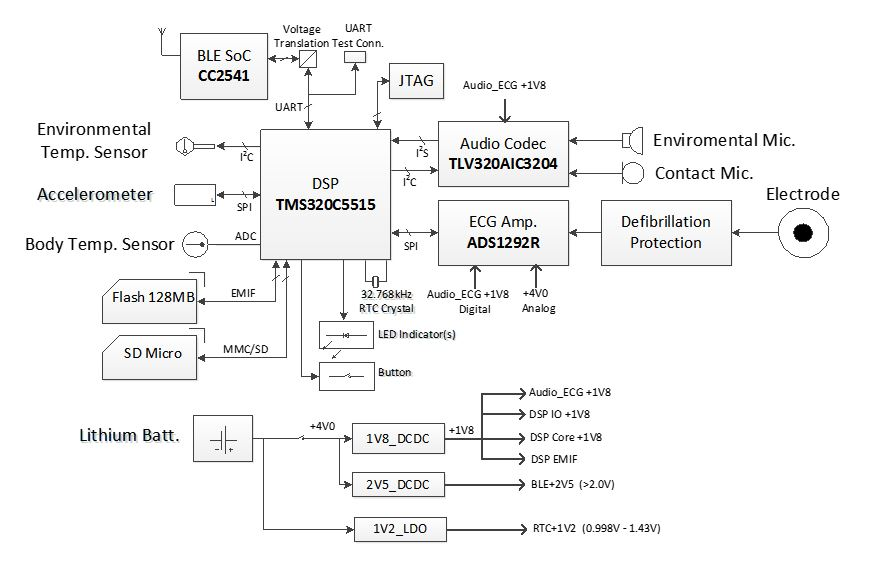
\includegraphics[scale = 0.75 ]{BlueBox_Architecture.JPG}
	\caption{BlueBox Hardware System Architecture\label{BlueBox_Architecture}}
\end{figure} 
\section{Digital Signal Processor}
TMS320C5515 is a fixed-point DSP is based on the TMS320C55x™ DSP generation CPU processor core. The C55x™ DSP architecture achieves high performance and low power through increased parallelism and total focus on power savings. Figure \ref{C5515 Architecture} shows the DSP architecture

\begin{figure}[h]
	\centering
	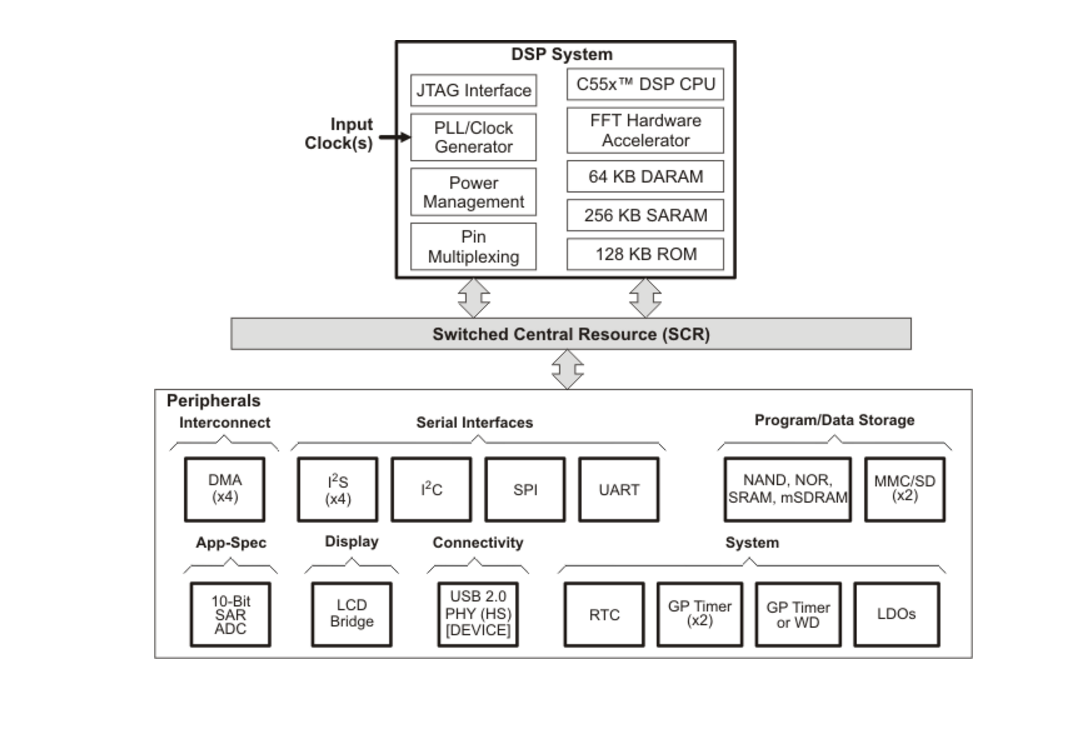
\includegraphics[scale = 0.75 ]{C5515 Architecture.PNG}
	\caption{DSP Architecture\label{C5515 Architecture}}
\end{figure} 
\subsection{Clock frequency}The DSP has a low power software programmable Phase Locked Loop(PLL) clock generator that  supports 60-,75-,100-,120-MHz clock rate.  
\subsection{On-Chip Memory}The DSP has 320K Bytes Zero-Wait state On-Chip RAM and 128K of On-Chip ROM

\subsection{Peripherals} The general-purpose input and output functions along with the 10-bit SAR ADC provide sufficient pins for status, interrupts, and bit I/O for LCD displays, keyboards, and media interfaces. Serial media is supported through two Multimedia Card/Secure Digital (MMC/SD) peripherals, four Inter-IC Sound (I2S Bus™) modules, one Serial-Port Interface (SPI) with up to 4 chip selects, one I2C multi-master and slave interface, and a Universal Asynchronous Receiver/Transmitter (UART) interface. 

\subsection{DMA} The device includes four Direct Memory Access(DMA) controllers, each with 4 channels, providing data movement for 16-independent channel contexts without CPU intervention. Each DMA controller can perform one 32-bit data transfer per cycle, in parallel and independent of the CPU activity.


\subsection{Power} Furthermore, the device includes three integrated LDOs (DSP LDO, ANA LDO, and USB LDO) to power different sections of the device. The DSP LDO can provide 1.3 V or 1.05 V to the DSP core (CVDD), 
selectable on-the-fly by software as long as operating frequency ranges are observed. 


\section{AIC3204 : Audio Codec}
TLV320AIC3204 is an analog interface chip (AIC) of TI company which is a flexible, low-power, low-voltage stereo audio codec with programmable inputs and outputs, PowerTune capabilities, fixed predefined and parameterizable signal-processing blocks, integrated PLL, integrated LDOs and flexible digital interfaces.  It has both recording and playback capabilities. The record part of the TLV320AIC3204 covers operations from 8kHz mono to 192kHz stereo recording, and contains programmable input channel configurations covering single-ended and differential setups, as well as floating or mixing input signals. It also includes a digitally-controlled stereo microphone preamplifier and integrated microphone bias. It integrates A / D and D / A conversion functions, it achieved high-precision A / D and D / A converter in the low-cost using Σ-△ technology. The size of the chip is very small and compact and its is available in  5 mm × 5 mm 32-pin QFN Package. 
As it has capabilities of recording stereo audio signals, it has two channels that it can record. We use one channel for respiration recording and the other for paramedic's log recording.

\section{ADS1292R : ECG Frontend}
ADS1292R is the ECG analog front end chip to which the electrode output is connected to.
ADS1292R is a two channel, simultaneous sampling, 24-bit, delta-sigma (ΔΣ) analog-to-digital converters (ADCs) with a built-in programmable gain amplifier (PGA), internal reference, and an onboard oscillator.  ADS1292R incorporate all features commonly required in portable, low-power medical electrocardiogram (ECG), sports, and fitness applications.With high levels of integration and exceptional performance, the ADS1292R enable the creation of scalable medical instrumentation systems at significantly reduced size, power, and overall cost. ADS1292R have a flexible input multiplexer per channel that can be independently connected to the internally-generated signals for test, temperature, and lead-off detection. Additionally, any configuration of input channels can be selected for derivation of the right leg drive (RLD) output signal. The ADS1292R operate at data rates from 500SPS up to 8 kSPS. The devices are packaged in a 5-mm × 5-mm, 32-pin thin quad flat pack (TQFP). Operating temperature is specified from –40°C to +85°C. ADS1292R is interfaced with the DSP through SPI.
 
\section{MPU9250 : Accelerometer sensor}
MPU-9250 is a 9-axis MotionTracking device that combines a 3-axis gyroscope, 3-axis accelerometer, 3-axis magnetometer and a Digital Motion Processor™ (DMP).With its dedicated I2C sensor bus, the MPU-9250 directly provides complete 9-axis MotionFusion™ output.MPU-9250 features three dedicated 16-bit analog-to-digital converters (ADCs) for digitizing each of the gyroscope outputs, accelerometer outputs, and magnetometer outputs. For precision tracking of both fast and slow motions MPU-9250 provides a user-programmable accelerometer full-scale range of ±2g, ±4g, ±8g, and ±16g. The package size down to a footprint and thickness of 3x3x1mm, to provide a very small yet high performance low cost package. 
\section{Temperature sensor}
\subsection{ STS21 : Environment temperature sensor}
STS21 is a low power, fully self calibrated digital temperature sensor well suited for applications with high demand on temperature accuracy. With dedicated I2C bus it directly provides the temperature output. The sensor comes in a package sized 3 x 3mm footprint and 1.1 mm height. 

\subsection{MA100: Body temperature sensor} 
MA100 is a Biomedical Chip Thermistor assemblies that are designed for use in applications involving both intermittent and continuous patient temperature monitoring. Although low in cost and small in size, these are highly stable, precision thermochips provide reliability, tight interchangeable tolerances, geometries, and fast response time that are often required. 
\section{Memory}
The BlueBox system has on-chip memory and the persistent micro SD card storage. Because a micro SD card is power intensive and takes hundreds of milliseconds to write to, the on-chip memory is used as buffer. Once there is enough buffer the data is written to the micro SD card and can be accessed by a computer. All the heavy lifting data transfer are done with the help of Direct Memory access peripheral interconnect to take off load from DSP. SD card is interfaced to DSP using MMC/SD interface. The SD card used for the application is a high capacity card that can support a maximum clock frequency of 50 MHz. These high capacity cards are not byte addressable. These high capacity cards are organized in 512 Byte sector or block and they are block addressable. In this thesis, the testing was done on kingston 8 GB micro SDHC card. 

\section{Battery and Power management circuitry}
 A GMB 302547 Lithium ion polymer rechargable battery is used to power the system. It has a capacity of 300 mAH at 3.7 V. The following picture shows the battery. It is 4 cm long , 2cm wide and 0.2 mm thick. And it weighs  8 grams. The battery is place on top of the central board housing. The central board has a battery charging circuitry that can charge the battery completely in 2 hours. The power management circuitry provides a powertrain that powers up the different power domain in the DSP  as shown in the system overview diagram above.             
%%% Local Variables: ***
%%% mode: latex ***
%%% TeX-master: "thesis.tex" ***
%%% End: ***
